\documentclass{article}

\usepackage{titlesec}
\usepackage{titling}
\usepackage[margin=1in]{geometry}
\usepackage{fontawesome}
\usepackage{tcolorbox}
\usepackage{graphicx}

\pagenumbering{gobble} 

\titleformat{\section}
{\normalfont\Large\bfseries}
{}
{0em}
{}
% [{\titlerule[0.8pt]}]

\titleformat{\subsection}
\setlength{\hoffset}{0.5em}
{\large\bfseries}
{}
{}
{}

\titleformat{\subsubsection}[runin]
{\bfseries}
{}
{0em}
{}

\titlespacing{\subsubsection}
{0em}{0em}{0em}

\setlength{\voffset}{-0.35in}
\setlength{\hoffset}{-0.75in}
\setlength{\headsep}{5pt}



\begin{document}
    \begin{minipage}[t]{5.5in\linewidth}
    \Huge\vspace{0in}\hspace{-0.30em}\textbf{Reshav Abraham}  

    \vspace{0em}\hspace{-0.2em}\Large\textbf{Full Stack ML Engineer} 

    \vspace{0.5em}\hspace{0em}\small\textbf{about me} 

        \begin{minipage}[t]{0.6\textwidth\hspace{0em}}
        I am a passionate software engineer interested in Full stack development
        and machine learning. I have experience building backend API's and Frontends. I also have experience in training and serving machine learning models. \par
        \end{minipage}
    \end{minipage}
    \begin{minipage}[t]{3in\linewidth\hspace{-2.3em}}
        \small
        \strut\vspace*{-\baselineskip}\newline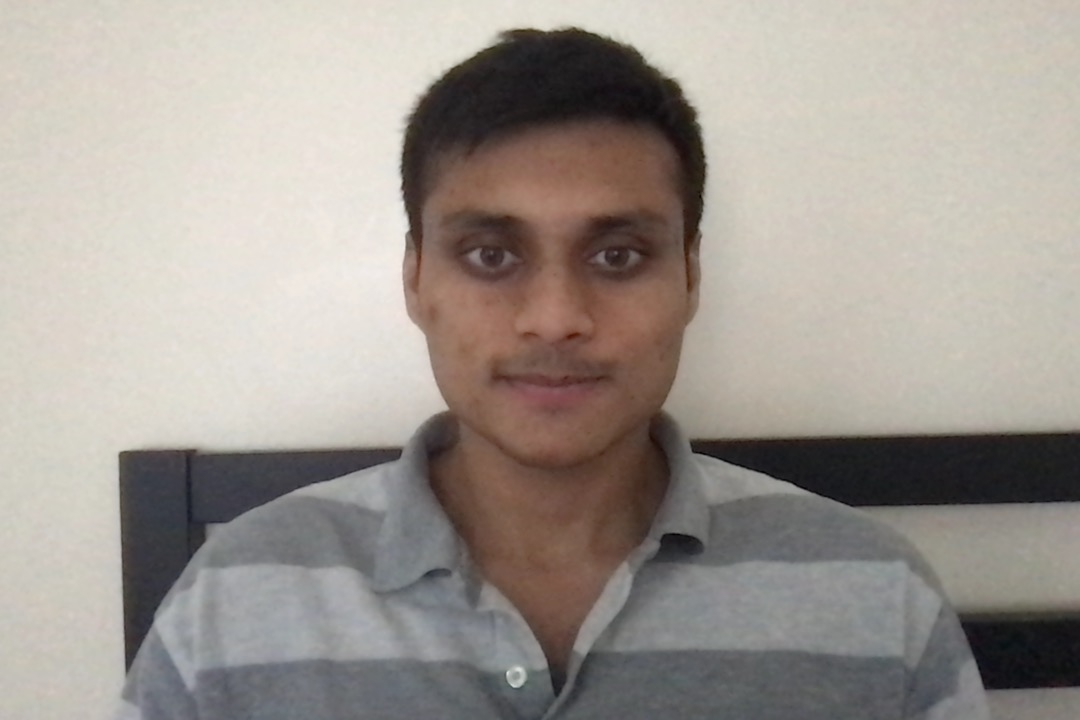
\includegraphics[width=1.4in]{reshav}

        \faEnvelopeO \, reshavabraham@gmail.com
        
        \faGithub\hspace \, https://github.com/reshav-abraham 

        \faLinkedin \, www.linkedin.com/in/reshav-abraham-ab8016a5

        \faHome \, 160 Vroom Street, Jersey City
    \end{minipage}

\vspace{1.3em}

\begin{minipage}[t]{0.45\textwidth\hspace{0in}}

    \section{\underline{Work Experience}}
        \vspace{-0.8em}
        \subsection{Nlmatics}
        % bfseries
        \vspace{-0.5em}\hspace{0.1em}
        \mdseries\bfseries{NLP Engineer}
        \vspace{0.1em}
        
        \hspace{0.5em}\mdseries\textrm{New York, NY | October 2019 - April 2021}

        \vspace{-0.8em}
        \begin{minipage}[t]{3.75in\textwidth\hspace{0in}}
            \vspace{0.3em}
            \hspace{1em}\textasteriskcentered \, \mdseries\textrm{Improved text indexing from PDF documents to enhance}
            
            \hspace{1.6em} search retrieval quality.
            
            \vspace{0.3em}
            \hspace{1em}\textasteriskcentered \, \mdseries\textrm{Designed back-end APIs with Python and Swagger.}

            \vspace{0.3em}
            \hspace{1em}\textasteriskcentered \, \mdseries\textrm{Built out front-end features with React and ANT design.}
            
            \vspace{0.3em}
            \hspace{1em}\textasteriskcentered \, \mdseries\textrm{Lead on-prem installation for clients and deploying on}

            \hspace{1.6em} restrictive environments.
            
            \vspace{0.3em}
            \hspace{1em}\textasteriskcentered \, \mdseries\textrm{Maintained and debugged CI/CD pipelines, with Docker}

            \hspace{1.6em} and Kubernetes.
        \end{minipage}

        \vspace{0.3em}
        \subsection{Dell EMC}
        % bfseries
        \vspace{-0.5em}\hspace{0.1em}
        \mdseries\bfseries{Software Intern}
        \vspace{0.1em}
        
        \hspace{0.5em}\mdseries\textrm{Charlotte, NC | May 2017 — August 2017}

        \vspace{-0.4em}
        \begin{minipage}[t]{3.75in\textwidth\hspace{0in}}
            \vspace{0.1em}
            \hspace{1em}\textasteriskcentered \, \mdseries\textrm{Optimized memory usage for enterprise data pipelining} 
            
            \hspace{1.6em} software by modeling a regression on real-time memory 
            
            \hspace{1.6em} consumption data using Apache Spark.
        \end{minipage}

        \section{\underline{Certificates}}
        \begin{minipage}[t]{3.75in\textwidth\hspace{0in}}            
            \mdseries\bfseries{Natural Language Processing with Deep Learning}
            
            \small\mdseries\textrm {CS224N, Stanford University, October 2020 — December 2020}
            
            \small\mdseries
            \vspace{0.2em}
            \hspace{1em}\textasteriskcentered \, \mdseries\textrm{Developed a Neural Machine Language Translation model in PyTorch.}
            
            \hspace{1em}\textasteriskcentered \, \mdseries\textrm{Implemented encoder and decoder networks using LSTM and CNN layers for processing out-of-vocabulary words.}
        \end{minipage}
        % \mdseries\textrm{CS224N, Stanford University, October 2020 — December 2020}
        % \begin{minipage}[t]{3.75in\textwidth\hspace{0in}}
        %     \mdseries\bfseries{Human Voice Detection}            
            
        %     \vspace{0.3em}
        %     \hspace{1em}\textasteriskcentered \, \mdseries\textrm{Developed a Neural Machine Language Translation model in Py-
        %     Torch.}

        %     \vspace{0.3em}
        %     \hspace{1em}\textasteriskcentered \, \mdseries\textrm{Implemented encoder and decoder networks using LSTM and CNN
        %     layers for processing out-of-vocabulary words.}
        
        % \end{minipage}

        \section{\underline{Projects}}
        \begin{minipage}[t]{3.75in\textwidth\hspace{0in}}
            \mdseries\bfseries{Human Voice Detection}            
            
            \vspace{0.3em}
            \small\mdseries
            \hspace{1em}\textasteriskcentered \, \mdseries\textrm{Developed a neural network architecture using CNN and linear layers
            for processing audio signals to identify human voices.}

            \vspace{0.3em}
            \hspace{1em}\textasteriskcentered \, \mdseries\textrm{Developed a script for scraping audio from YouTube playlists.}
            
            \vspace{0.3em}
            \hspace{1em}\textasteriskcentered \, \mdseries\textrm{Utilized MFCC and other signal processing techniques to prepare
            data.}

        \end{minipage}

\end{minipage}
    \begin{minipage}[t]{3in\linewidth\hspace{0.95in}}
    \section{\underline{Technical Skills}}
    \vspace{-0.7em}
    \subsubsection{Programming}
    \, Python, JS, Docker, Kubernetes
    \vspace{0.3em}

    \subsubsection{Frameworks}
    \, PyTorch, Tensorflow, Swagger, \, \, React
    \vspace{0.3em}

    \subsubsection{Coud}
    \, GCP, Azure
    \vspace{0.3em}
    
    \subsubsection{Databases}
    \, MongoDB, Postgress, Redis}

    \subsubsection{Markup}
    \, {\LaTeX}, HTML, CSS}

    \vspace{4em}
    \section{\underline{Education}}
    \large\bfseries{B.S Computer Engineering}

    \bfseries{Purdue University} 

    \small\mdseries\textrm West Lafayette, IN | 2014 — 2018

    \vspace{0.4em}

    \small\bfseries\textrm{Multi-core Processor System Verilog}
    
    \vspace{0.3em}
    \small\mdseries
    \hspace{0em}\textasteriskcentered \, \mdseries\textrm{Implemented a synthesizable multi-core processor for processing MIPS assembly language in SystemVerilog.}

    \small\bfseries\textrm{Automated Nerf-Gun Turret}
    
    \vspace{0.3em}
    \small\mdseries
    \hspace{0em}\textasteriskcentered \, \mdseries\textrm{Engineered a turret gun that detects human targets and shoots Nerf darts at them.}

    \vspace{0.5em}
    \hspace{0em}\textasteriskcentered \, \mdseries\textrm{Designed a human-target detection algorithm with MobileNetSSD and OpenCV.}

    \vspace{10em}
    \begin{minipage}[t]{3.75in\textwidth\hspace{0in}}
        \large\mdseries\bfseries{Interests}            
        
        \small\mdseries
        \vspace{0.3em}
        \hspace{0.3em}\textasteriskcentered \, \small\mdseries\textrm{Soccer}

        \vspace{0.3em}
        \hspace{0.3em}\textasteriskcentered \, \small\mdseries\textrm{Guitar}        
        
        \vspace{0.3em}
        \hspace{0.3em}\textasteriskcentered \, \small\mdseries\textrm{Chess}

    \end{minipage}

\end{minipage}


\end{document}